\documentclass[a4paper,12pt]{article}
\usepackage[english]{babel}
\usepackage[utf8]{inputenc}
\usepackage{fontspec}
\setmainfont{CMU Serif}

\newfontfamily{\englishfont}{CMU Serif}
\newfontfamily{\thaifont}[Scale=MatchUppercase]{TH Sarabun Chula}
\newenvironment{thailang}{\thaifont}

\usepackage[Latin,Thai]{ucharclasses}
\setTransitionTo{Thai}{\thaifont}
\setTransitionFrom{Thai}{\englishfont}

\XeTeXlinebreaklocale "th_TH"
\XeTeXlinebreakskip = 0pt plus 1pt 

\usepackage{setspace}
\onehalfspacing

\usepackage{amsmath,amsthm,amssymb}
\usepackage{physics}
\usepackage[margin=1in]{geometry}
\usepackage{graphicx}

\title{การประมาณในฟิสิกส์}
\author{อิธิพัฒน์ ธนบดีกาญจน์}

\begin{document}

\maketitle

\section{บทนำ}

วิชาฟิสิกส์ เป็นวิชาที่กำเนิดขึ้นเพื่ออธิบายและทำนายปรากฏการณ์ต่าง ๆ โดยส่วนใหญ่จะนำคณิตศาสตร์มาประยุกต์ใช้แต่ในบางครั้งการพิจารณาปรากฏการณ์นั้น ซับซ้อนมากเกินไปจนไม่สามารถคำนวณได้ง่ายและจินตนาการสถานการณ์จากสมการได้ยาก จึงทำให้มีการประมาณเกิดขึ้นโดยการประมาณนี้อาจจะไม่ถูกใจนักคณิตศาสตร์มากนักเพราะทำให้เกิดความคลาดเคลื่อน แต่ในวิชาฟิสิกส์นั้นเป็นการพิจารณาสถานการณ์จริง โดยใช้ข้อมูลจากการวัดจริง ๆ ซึ่งในทางปฏิบัติ การวัดนั้นมีความคลาดเคลื่อนในตัวอยู่แล้วและในหลาย ๆ ครั้ง การประมาณนั้นคลาดเคลื่อนน้อยกว่าความคลาดเคลื่อนของค่าที่เราวัดได้ด้วยซ้ำ

\section{รูปแบบการประมาณ}
ผู้เขียนจะเสนอตัวอย่างในฟิสิกส์ระดับมัธยมปลายเท่านั้น ในความเป็นจริงการประมาณนั้นมีหลากหลายรูปแบบมาก แต่มีจุดประสงค์เดียวกันคือ ทำให้การวิเคราะห์สถานการณ์มีประสิทธิภาพมากขึ้น
	\subsection{Simple Pendulum}
	การประมาณรูปแบบนี้ใช้ประโยชน์จาก Taylor series
	\begin{figure}[h]
		\centering
		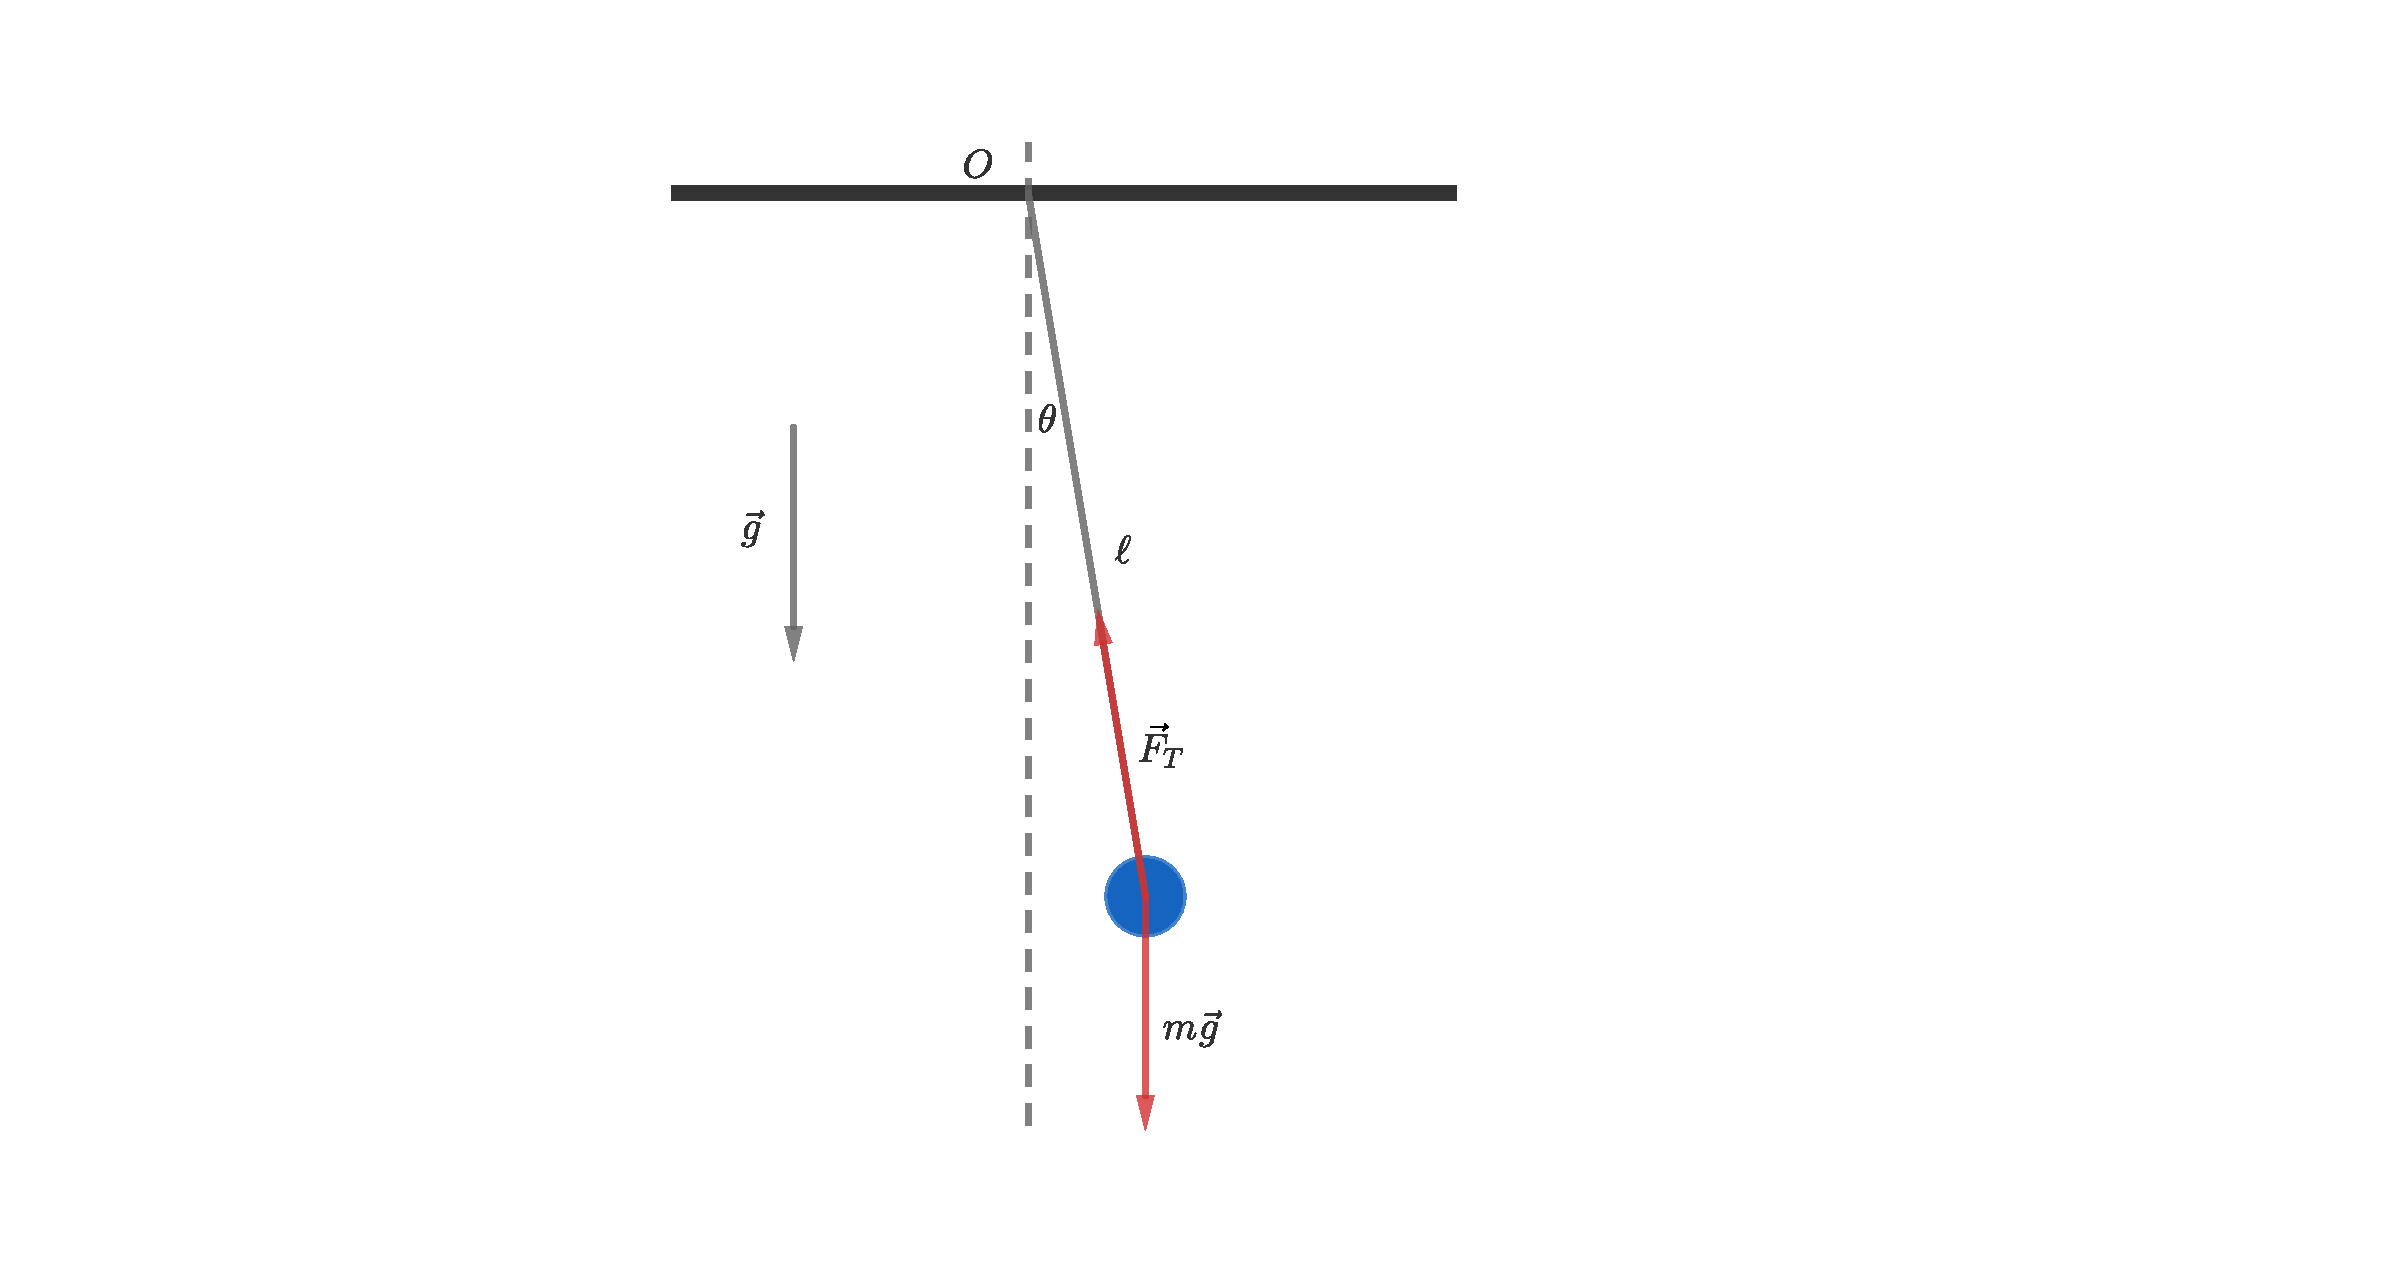
\includegraphics[width=0.3\linewidth]{pendulum}	
		\label{fig:pen1}
	\end{figure}
\pagebreak
	\subsubsection{การหาคาบของ Simple Pendulum}
	จากสมการทอร์ก
	
	$$\sum\vec{\tau}=\dv{\vec{L}}{t}$$
	คิดทอร์กรอบทุก $O$ จะได้
	\begin{equation}
	\vec{\tau}_{F_T}+\vec{\tau}_{m\vec{g}}=\dv{t}(I\vec{\omega})
	\end{equation}
	ให้ $\vec{\ell}$ เป็นเวกเตอร์ที่ชี้จากจุด $O$ ไปยังมวล $m$
	$$\vec{0}+\vec{\ell}\times m\vec{g}=I\dv{t}\vec{\omega}$$
	ให้ $\hat{k}$ มีทิศพุ่งเข้ากระดาษ
	$$-(\ell mg\sin\theta\hat{k})=I(\dv{t}\omega)\hat{k}$$
	ต้องมีเครื่องหมายลบเนื่องจากแรง $m\vec{g}$ เมื่อแตกเวกเตอร์เข้าแกนสัมผัสการเคลื่อนที่จะชี้ไปทางซ้าย โดยเราให้ทางขวาเป็นบวก
	$$-\ell mg\sin\theta=I\alpha$$
	หาโมเมนต์ความเฉื่อยรอบ $O$ จะได้ $I=m\ell^2$\\
	$$-\ell mg\sin\theta=(m\ell^2)\alpha$$
	$$-\frac{g}{\ell}\sin\theta=\alpha$$
	เนื่องจากสมการลักษณะนี้ไม่ใช่ SHM\footnote{Simple harmonic motion} เราจึงใช้ Taylor series ประมาณ
	\begin{equation}
	\sin\theta\approx\theta
	\end{equation}
	โดยเราเรียกการประมาณรูปแบบนี้ว่า Small-angle approximation หรือเป็นการประมาณเมื่อมุมมีค่าน้อย ๆ ในหน่วย radian
	\begin{equation}\label{pen_shm}
	\boxed{
		-\frac{g}{\ell}\theta=\alpha
	}
	\end{equation}
	จากสมการที่ (\ref{pen_shm}) จะได้
	$$\omega=\sqrt{\frac{g}{\ell}}$$
	จาก
	$$T=\frac{2\pi}{\omega}$$
	จะได้
	\begin{equation}\label{ppen}
	\boxed{
		T=2\pi\sqrt{\frac{\ell}{g}}
	}
	\end{equation}
\linebreak
	จากสมการที่ (\ref{ppen}) เราจะรู้สึกคุ้นมากเนื่องจากเป็นสูตรหาคาบของเพนดูลัมอย่างง่ายที่จำกันในระดับมัธยมปลาย แต่รู้หรือไหมว่ามันเป็นการประมาณไม่ใช่สูตรที่ให้ค่าแม่นตรง!
	\subsubsection{ความใกล้เคียงของการใช้ Small-angle approximation}
	เนื่องจากการหาค่า $\sin\theta$ โดย Taylor series จะได้
	\begin{equation}\label{taylor_sinx}
	\sin\theta=\theta-\frac{\theta^3}{3!}+\frac{\theta^5}{5!}-\frac{\theta^7}{7!}+\dots
	\end{equation}
	แต่เราต้องการเพียงแค่พจน์ที่ 1 (อันดับ1)เพื่อให้ได้สมการเป็นการเคลื่อนที่แบบ SHM ซึ่งถ้าเราสังเกตพจน์ที่ 2 เป็นต้นไปจะพบว่ามีการหารด้วยแฟกทอเรียล ซึ่งมีค่ามากขึ้นอย่างรวดเร็วเมื่อเลขมีค่ามากขึ้น ดังนั้นจะทำให้พจน์ต่อ ๆ ไปมีค่าน้อยมาก ๆ\\
	\begin{figure}[h]
		\centering
		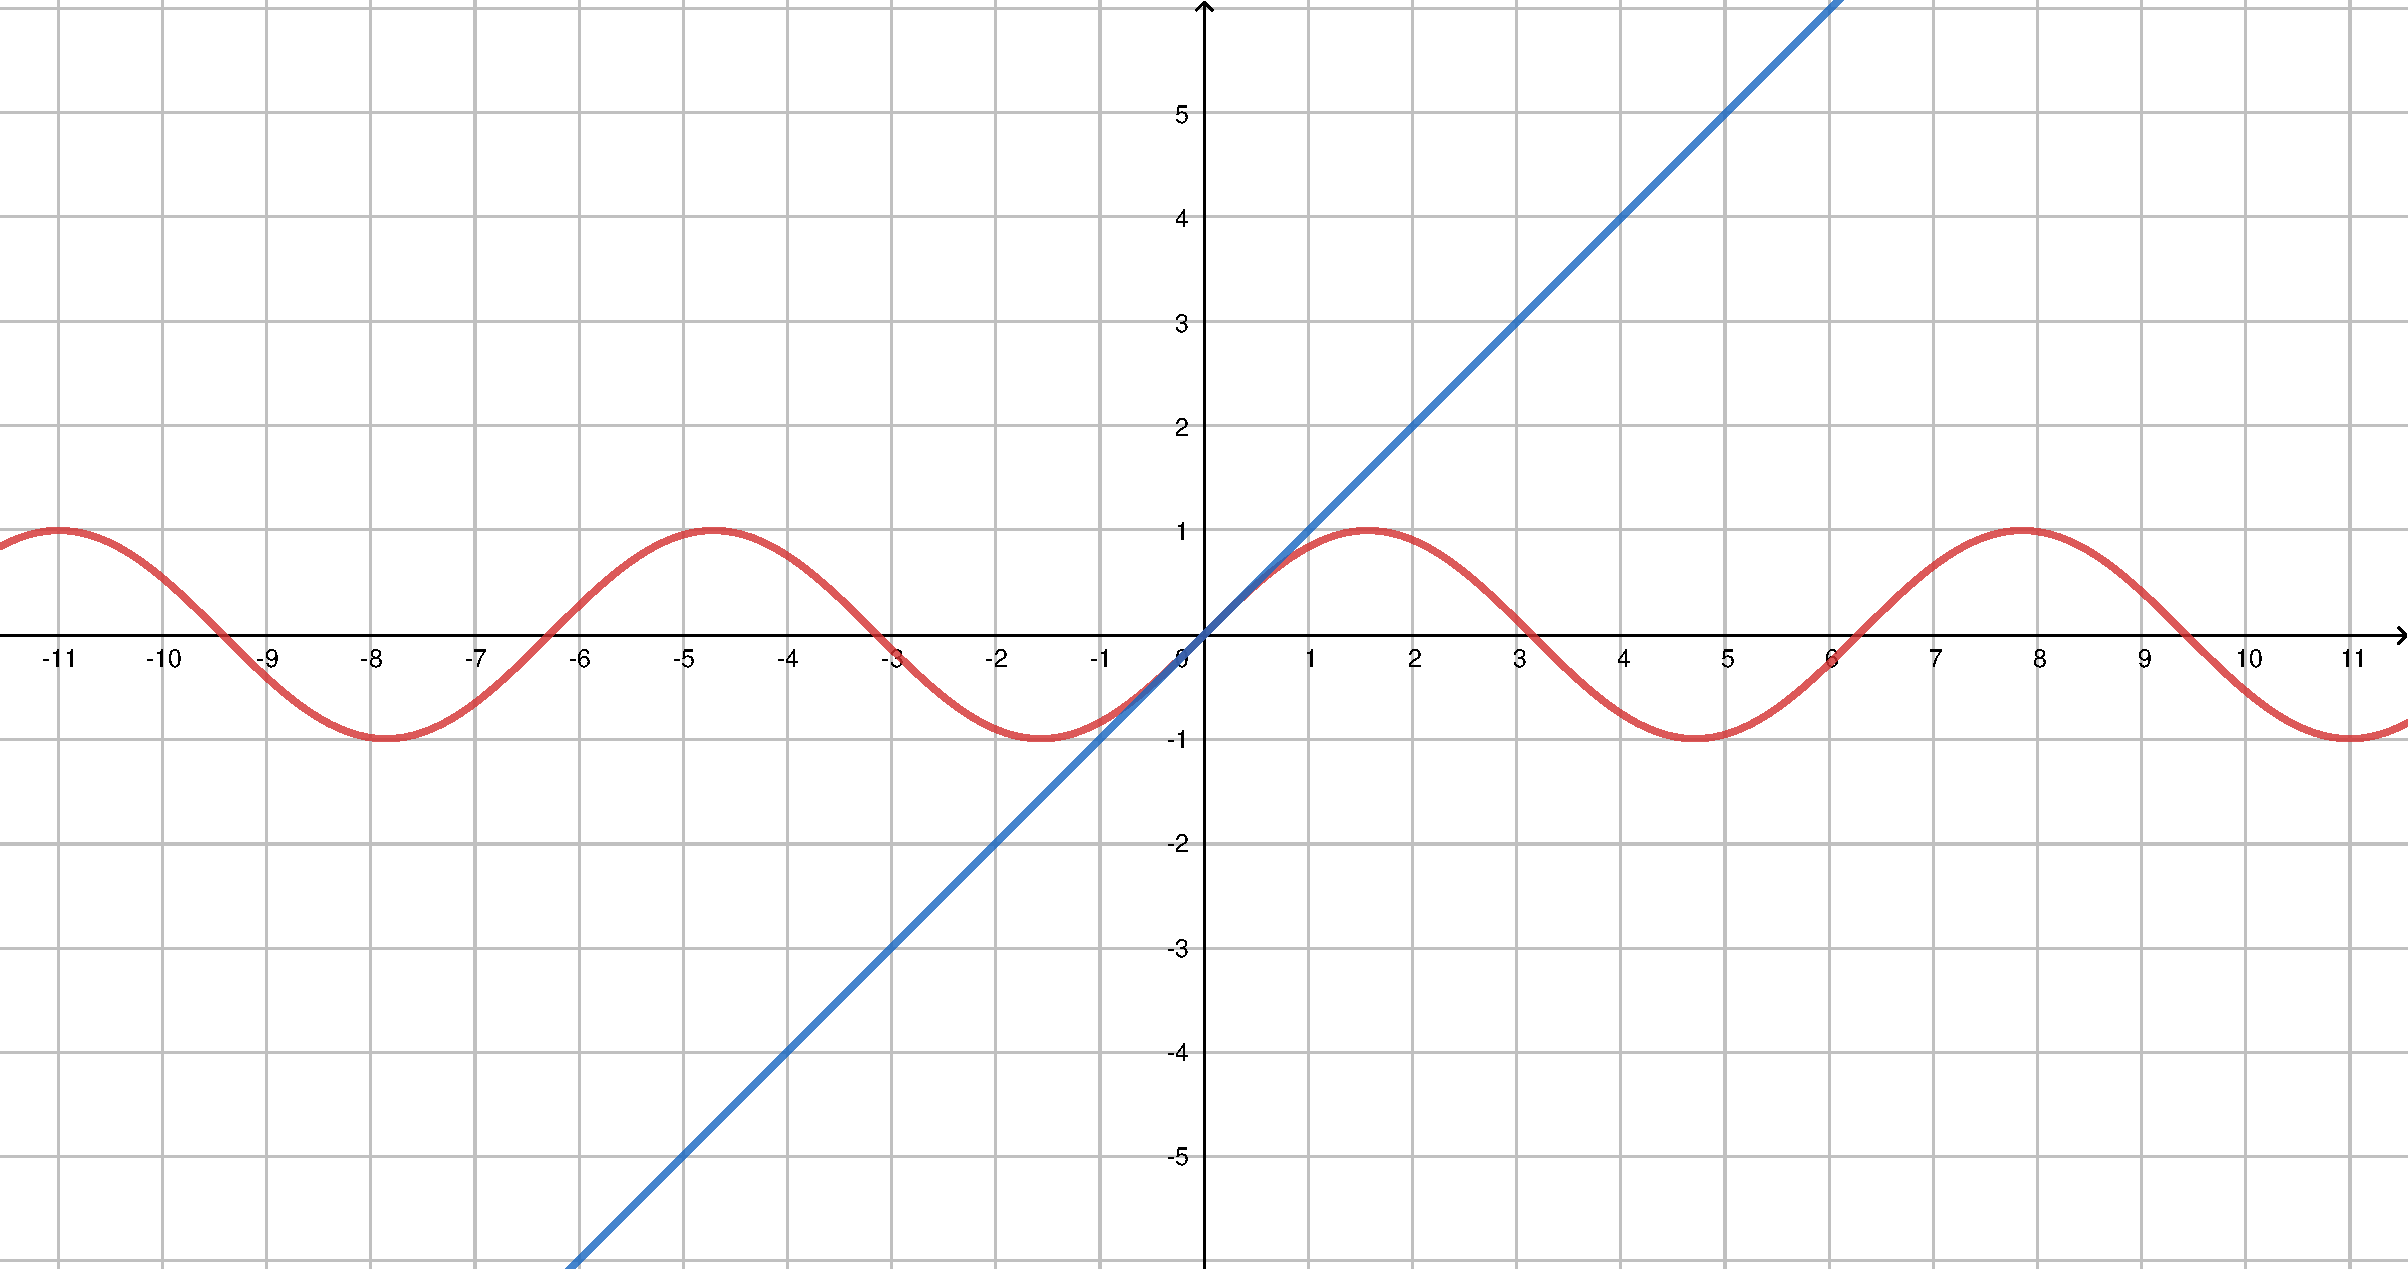
\includegraphics[width=0.8\linewidth]{plot_sinx_x}	
		\label{fig:plot1}
		\caption{สีแดง:$y=\sin \theta$ สีฟ้า:$y=\theta$}
	\end{figure}
\linebreak
	จะสังเกตได้ว่า กราฟจะใกล้กันเมื่อค่า $\theta$ น้อย ๆ โดย $\sin x\approx x$ มีความคลาดเคลื่อน $1\%$ ที่ $\theta$ ประมาณ 0.244 rad หรือ $14^\circ$\\
	\indent สมมติเราแกว่ง Simple Pendulum ด้วยมุม $10.0^\circ$ หรือประมาณ $0.175$ rad\\
	คำนวณค่า $\sin$ ได้
	$$\sin10.0^\circ\approx0.174\;\mathrm{rad}$$
	ถ้าพิจารณาเลขนัยสำคัญจะเห็นได้ว่าคลาดเคลื่อนเพียง 0.001 rad ซึ่งถือว่าเป็นการประมาณที่ดีมาก ในการทดลองจริง 0.001 rad มีค่าประมาณ $0.06^\circ$ ซึ่งมีค่าน้อยมากเมื่อเทียบความแม่นยำเครื่องมือที่ใช้ทดลองทั่วไป (การที่ค่า $\theta$ ห่างจากค่า $\sin\theta$ มากจะทำให้ค่า $T$ ที่ได้จาก $T=2\pi\sqrt{\frac{\ell}{g}}$ คลาดเคลื่อนมาก)
	\subsection{เสียง}
	การประมาณรูปแบบนี้ใช้ประโยชน์จาก Binomial expansion\footnote{ความจริงแล้วเป็นส่วนหนึ่งของ Taylor series แต่ผู้เขียนเห็นว่ามีความเด่นในวิชาฟิสิกส์เป็นพิเศษจึงแยกออกมาจาก Taylor series} 
	\subsubsection{การหาอัตราเร็วของเสียงในอากาศ}
	
	ถึงแม้การหาอัตราเร็วของเสียงนั้นมีการประมาณหลายอย่างและเป็นเหตุการณ์ที่ค่อนข้างอุดมคติ ก็ถือว่าเป็นการประมาณที่ดีพอที่จะนำไปใช้งานจริง
	
	เนื่องจากการพิสูจน์ที่มาของ 2 สูตรที่จะกล่าวถึงนี้ต้องใช้ความรู้คณิตศาสตร์ค่อนข้างมากและจะนอกเหนือจุดประสงค์ของเอกสารนี้มากเกินไป ผู้เขียนจึงขอยกสูตรมาใช้เลย
	\begin{equation}\label{v_s}
	v=\sqrt{\frac{B_{adia}}{\rho}}
	\end{equation}
	\begin{equation}\label{B_a}
	B_{adia}=\gamma P
	\end{equation}
	นำ (\ref{B_a}) แทนใน (\ref{v_s}) จะได้
	\begin{equation}\label{v_s2}
	v=\sqrt{\frac{\gamma P}{\rho}}
	\end{equation}
	จากกฎของแก๊สอุดมคติ
	\begin{equation}
	PV=nRT
	\end{equation}
	$$PV=(\frac{m_t}{\mathcal{M}})RT$$
	$$P\mathcal{M}=(\frac{m_t}{V})RT$$
	$$P\mathcal{M}=\rho RT$$
	\begin{equation}\label{rho_a}
	\rho=\frac{P\mathcal{M}}{RT}
	\end{equation}
	นำ (\ref{rho_a}) แทนใน (\ref{v_s2}) จะได้
	$$v=\sqrt{\frac{\gamma P}{\frac{P\mathcal{M}}{RT}}}$$
	\begin{equation}\label{v_s3}
	\boxed{
		v=\sqrt{\frac{\gamma RT}{\mathcal{M}}}
	}
	\end{equation}
	ในระดับมัธยมสูตรที่เราคุ้นตา คือ $v=331+0.6T$ เมื่อ $T$ มีหน่วยเป็นองศาเซลเซียส ซึ่งเราสามาถสร้างได้จากสมการ (\ref{v_s3}) แต่ $T$ ในสมการ (\ref{v_s3}) มีหน่วยเป็นเคลวินจึงต้องใช้ความสัมพันธ์
	$$T_\mathrm{K}\approx T_{^\circ \mathrm{C}}+273$$
	จะได้
	$$v=\sqrt{\frac{\gamma R(T_{^\circ \mathrm{C}}+273)}{\mathcal{M}}}$$
	หลังจากนี้ผู้เขียนจะเขียน $T_{^\circ \mathrm{C}}$ เป็น $T$ เพื่อความสะดวก
	$$v=\sqrt{\frac{\gamma R}{\mathcal{M}}}{\sqrt{T+273}}$$
	$$v=\sqrt{\frac{273\gamma R}{\mathcal{M}}}{\sqrt{\frac{T}{273}+1}}$$
	จัดรูปเล็กน้อยเพื่อให้เห็นรูปแบบที่จะถูกประมาณอย่างชัดเจน
	\begin{equation}\label{v_sb}
	v=\sqrt{\frac{273\gamma R}{\mathcal{M}}}\left(1+\frac{T}{273}\right)^{1/2}
	\end{equation}
	เพราะสูตรในการหาอัตราเร็วนี้มีการหากรณฑ์ที่สองของตัวแปร $T$ ที่ไม่ใช่ค่าคงที่ของสถานการณ์ที่เราสนใจ จึงใช้ Binomial expansion แก้ปัญหานี้ โดยประมาณ
	$$\left(1+\frac{T}{273}\right)^{1/2}\approx1+\frac{1}{2}\left(\frac{T}{273}\right)$$
	โดยเราเรียกการประมาณรูปแบบนี้ว่า Binomial approximation และจะได้
	\begin{equation}\label{v_s4}
	v\approx\sqrt{\frac{273\gamma R}{\mathcal{M}}}\left(1+\frac{1}{2}\left(\frac{T}{273}\right)\right)
	\end{equation}
	เนื่องจากองค์ประกอบหลักของอากาศคือ ไนโตรเจน $\approx 78\%$ ออกซิเจน $\approx 21\%$ และอาร์กอน $\approx 1\%$ ดังนั้น
	$$\mathcal{M}_{air}\approx29.0\;\mathrm{g/mol}\approx29.0\times10^{-3}\;\mathrm{kg/mol}$$
	และเนื่องจากอากาศส่วนใหญ่บนโลกของเราประกอบด้วยแก๊สอะตอมคู่ ($\mathrm{N_2,O_2}$) เราจะประมาณให้ $\gamma=\frac{7}{5}$
	จากนั้นนำค่าที่ได้แทนใน (\ref{v_s4})
	$$v\approx\sqrt{\frac{273(7/5)(8.314)}{29.0\times10^{-3}}}\left(1+\frac{T}{546}\right)$$
	$$v\approx331\left(1+\frac{T}{546}\right)$$
	$$v\approx331+0.606T$$
	ถ้าประมาณให้หยาบกว่านี้ก็จะได้ค่าเหมือนที่ท่องกันในระดับมัธยม คือ
	\begin{equation}\label{v_sf}
	\boxed{
	v=331+0.6T
	}
	\end{equation}
	\subsubsection{ความใกล้เคียงของการใช้ Binomial approximation}
	การกระจายพจน์ $(1+x)^n$ ด้วย Binomial approximation จะได้
	\begin{equation}
	(1+x)^n=\sum_{k=0}^{\infty}{n\choose k}x^k=1+nx+\frac{n(n-1)}{2!1!}x^2+\dots
	\end{equation}
	แต่เพราะเราต้องการประสิทธิภาพในการคำนวณ โดยทั่วไปแล้วจะประมาณเป็น $1+nx$ ก็ให้ความแม่นยำที่เพียงพอ เมื่อ $\abs{x}\ll1$\\
	\begin{figure}[h]
		\centering
		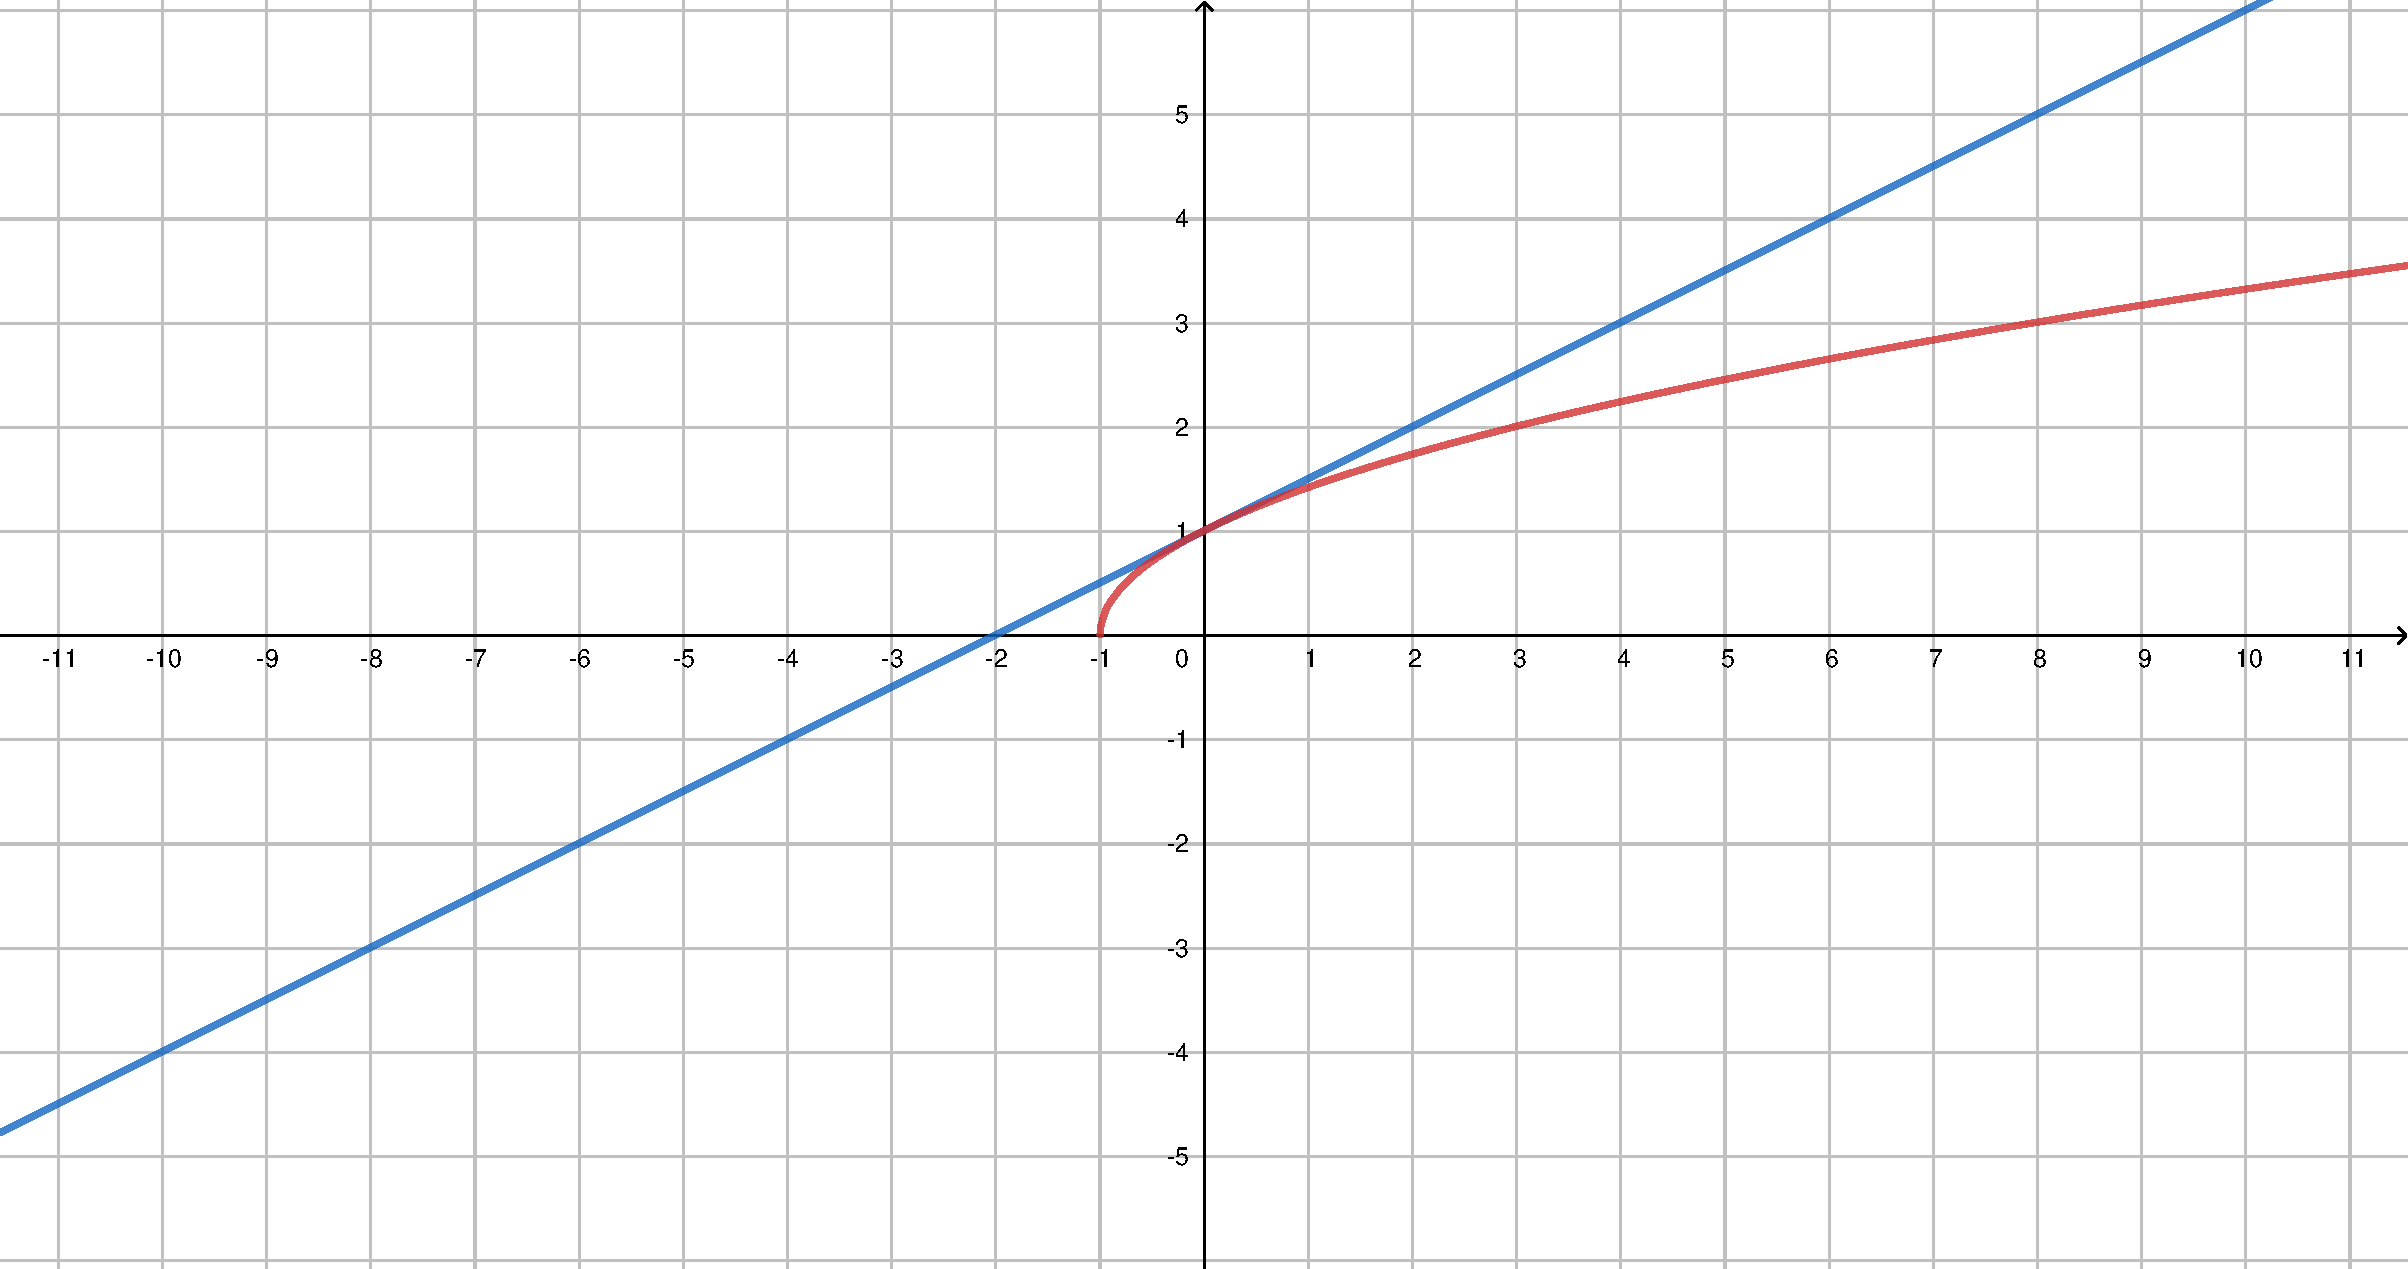
\includegraphics[width=0.8\linewidth]{plot_binomial}	
		\label{fig:plot2}
		\caption{สีแดง:$y=(1+x)^{1/2}$ สีฟ้า:$y=1+\frac{1}{2}x$}
	\end{figure}
\linebreak
	เราสมมติให้ $n=\frac{1}{2}$ ก็จะเห็นว่ากราฟจะใกล้กันเมื่อ $\abs{x}\ll1$\\
	\indent สมมติเราหาอัตราเร็วของเสียงในอากาศอุณหภูมิ $30^\circ \mathrm{C}$
	แทนในสูตร (\ref{v_sf}) จะได้ $v= 349$ m/s และแทนในสูตร (\ref{v_sb}) จะได้ $v\approx 348.73$ m/s คำนวณเปอร์เซ็นต์ความคลาดเคลื่อนได้
	$$\mathrm{Error}=\frac{\abs{348.73-349}}{349}\times100\%\approx 0.08\%$$
	แสดงว่าที่อุณหภูมิ $30^\circ \mathrm{C}$ มีความคลาดเคลื่อนของอัตราเร็วของเสียงในอากาศเพียง 0.08\% เมื่อใช้ \\Binomial approximation และจะเห็นได้ว่าการประมาณในรูปแบบนี้มีความแม่นยำที่สูงมากและเพียงพอที่จะนำผลไปใช้ในทางปฏิบัติทั่ว ๆ ไป
\end{document}